%========================
% Theme
%========================
\documentclass[8pt]{beamer}
\setbeamersize{text margin left=10mm,text margin right=10mm} 
\usetheme[progressbar=frametitle]{metropolis}
\usepackage{appendixnumberbeamer} % handles appendix slide numbering

%========================
% Packages: Icons and Tables
%========================
\usepackage{booktabs}        % professional tables
\usepackage[scale=1]{ccicons} % Creative Commons icons

%========================
% Packages: Plots and TikZ
%========================
\usepackage{pgfplots}
\usepgfplotslibrary{dateplot}

\usepackage{tikz}
\usetikzlibrary{positioning}

%========================
% Packages: Algorithms
%========================
\usepackage{algorithm}
\usepackage{algpseudocode}

%========================
% Packages: Math
%========================
\usepackage{amsmath,amsfonts,amsthm,amssymb}
\newtheorem{prop}{Proposition}

%========================
% Custom commands
%========================
\usepackage{xspace}
\newcommand{\themename}{\textbf{\textsc{metropolis}}\xspace}

%========================
% Custom footline
%========================
\setbeamertemplate{footline}
{%
  \leavevmode%
  \hbox{%
  \begin{beamercolorbox}[wd=.35\paperwidth,ht=2.5ex,dp=1.5ex,center]{author in head/foot}%
    \usebeamerfont{author in head/foot}\insertshortauthor
  \end{beamercolorbox}%
  \begin{beamercolorbox}[wd=.3\paperwidth,ht=2.5ex,dp=1ex,center]{title in head/foot}%
    \usebeamerfont{title in head/foot}\insertshorttitle
  \end{beamercolorbox}%
  \begin{beamercolorbox}[wd=.3\paperwidth,ht=2.5ex,dp=1ex,right]{date in head/foot}%
    \usebeamerfont{date in head/foot}\insertframenumber{} / \inserttotalframenumber
  \end{beamercolorbox}}%
  \vskip0pt%
}

%========================
% Remove default navigation symbols
%========================
\setbeamertemplate{navigation symbols}{}

\usepackage{pgf,pgfarrows,pgfnodes,pgfautomata,pgfheaps,pgfshade}
\usepackage{hyperref}
\usepackage{listings}
\usepackage{color}

\lstset{language=R,
    basicstyle=\small\ttfamily,
    stringstyle=\color{DarkGreen},
    otherkeywords={0,1,2,3,4,5,6,7,8,9},
    morekeywords={TRUE,FALSE},
    deletekeywords={data,frame,length,as,character},
    keywordstyle=\color{blue},
    commentstyle=\color{DarkGreen},
}

\usepackage{xcolor}

\lstset{
    language=Python,
    basicstyle=\ttfamily\small,
    keywordstyle=\color{blue},
    commentstyle=\color{gray},
    stringstyle=\color{red},
    breaklines=true,
    numbers=left,
    numberstyle=\tiny
}



%%%%%%%%%%%%%%%%%%%%%%%%%%%%%%%%%%%%%%%%%%%%%%%%%%%%%%%%%%%%%%%%%%%%
%%%%%%%%%%%%%%%%%%%%%%%%%%%%%%%%%%%%%%%%%%%%%%%%%%%%%%%%%%%%%%%%%%%%
% AQUI SE DEFINEN LAS IMAGENES PARA UTILIZAR DESPUES
%\pgfdeclareimage[interpolate=true, height=7cm,width=16cm]{halton-points}{halton-points}
%\pgfdeclareimage[interpolate=true, height=3cm, width =4cm]
%{serie-petroleo-reducido}{serie-petroleo-reducido}
%\pgfdeclareimage[interpolate=true, height=3cm, width =4cm]{rectangle-triangle}{rectangle-triangle}
%\pgfdeclareimage[interpolate=true, height=3cm, width =4cm]{any-angle}{any-angle}
%\pgfdeclareimage[interpolate=true, height=3cm, width =4cm]{Pythagoras}{Pythagoras}


\title{Chapter 1 - Random Number Generation}
\subtitle{Conditional Distributions}
\author{Prof. Alex Alvarez, Ali Raisolsadat}
\institute{School of Mathematical and Computational Sciences \\ University of Prince Edward Island}
\date{} % leave empty or add \today
%\title[Stat 4110]{Stat 4110 Statistical Simulation}
%\subtitle{}
%\author[University of Prince Edward Island]{School of Mathematical and Computational Sciences \\ University of Prince Edward Island}

%========================
% Begin document
%========================
\begin{document}

%-------------------
% Title frame
%-------------------
\maketitle

%-------------------
% Slide 1: Conditional Distributions
%-------------------
\begin{frame}{Conditional Distributions}
\textbf{Conditional Distribution}: Suppose that we we start with a random variable $X$ with a distribution $P_X$ that we know how to sample from. Let $A$ be an event and consider the conditional distribution of $X$ given $A$ $P_{X|X\in A}$.

\vspace{2mm}

We will be able to sample from the conditional distribution $P_{X|X\in A}$ by using a version of the rejection sampling algorithm as follows:

\vspace{2mm}

\alert{Algorithm}
\begin{enumerate}
\item Generate $X \sim P_X$ (proposal)
\item If $X \in A$ then $Y=X$ (proposal is accepted)
\item If $X \notin A$ then return to step 1
\item Return Y
\end{enumerate}
\end{frame}

%-------------------
% Slide 2: Conditional Distributions Example
%-------------------
\begin{frame}[fragile]{Conditional Distributions Example}
\textbf{Example} Generate a random sample of size $n=1000$ from the conditional distribution of $X \sim N(0,1) $  conditioned on $X\geq 0$

\vspace{2mm}

\alert{Code}
\begin{columns}
\column{0.45\textwidth}
\textbf{R Code}

\begin{lstlisting}
n <- 1000
counter <- 1 

target_sample <- vector();
while (counter < n+1) { 
  proposal <-rnorm(1)
  
  if (proposal > 0){
    target_sample[counter] <- proposal
    counter <- counter+1
  }
}  
hist(target_sample) 
\end{lstlisting}

\column{0.50\textwidth}
\textbf{Python Code}:
\begin{lstlisting}
import numpy as np
import matplotlib.pyplot as plt

n = 1000
counter = 0
target_sample = []
mu, sigma = 0, 1

while counter < n:
    proposal = np.random.normal(loc=mu, scale=sigma)
    if proposal > 0:
        target_sample.append(proposal)
        counter += 1
        
plt.hist(target_sample, bins=30)
plt.show()
\end{lstlisting}
\end{columns}
\end{frame}

%-------------------
% Slide 3: Conditional Distributions Example
%-------------------
\begin{frame}[fragile]{Conditional Distributions Example (Vectorized)}
\textbf{Example}: Generate a random sample of size $n=1000$ from the conditional distribution of $X \sim N(0,1) $ conditioned on $X\geq 0$

\vspace{2mm}

\alert{Code}
\begin{columns}
\column{0.45\textwidth}
\textbf{R Code}

\begin{lstlisting}
n <- 1000
mu <- 0
sigma <- 1
samples <- 
   rnorm(n * 2, mean = mu, sd = sigma)
target_sample <-
   samples[samples > 0]
target_sample <- 
   target_sample[1:n]
hist(target_sample, breaks = 30)
\end{lstlisting}

\column{0.50\textwidth}
\textbf{Python Code}

\begin{lstlisting}
import numpy as np
import matplotlib.pyplot as plt

n = 1000
mu, sigma = 0, 1
samples =
     np.random.normal(loc=mu, scale=sigma, size=n*2) 
target_sample = 
     samples[samples > 0]                        
target_sample = target_sample[:n]                         

plt.hist(target_sample, bins=30)
plt.show()
\end{lstlisting}

\end{columns}
\end{frame}


%-------------------
% Slide 4: Conditional Distributions Example Plot
%-------------------
\begin{frame}{Uniform sampling from a rectangle}
\begin{center}
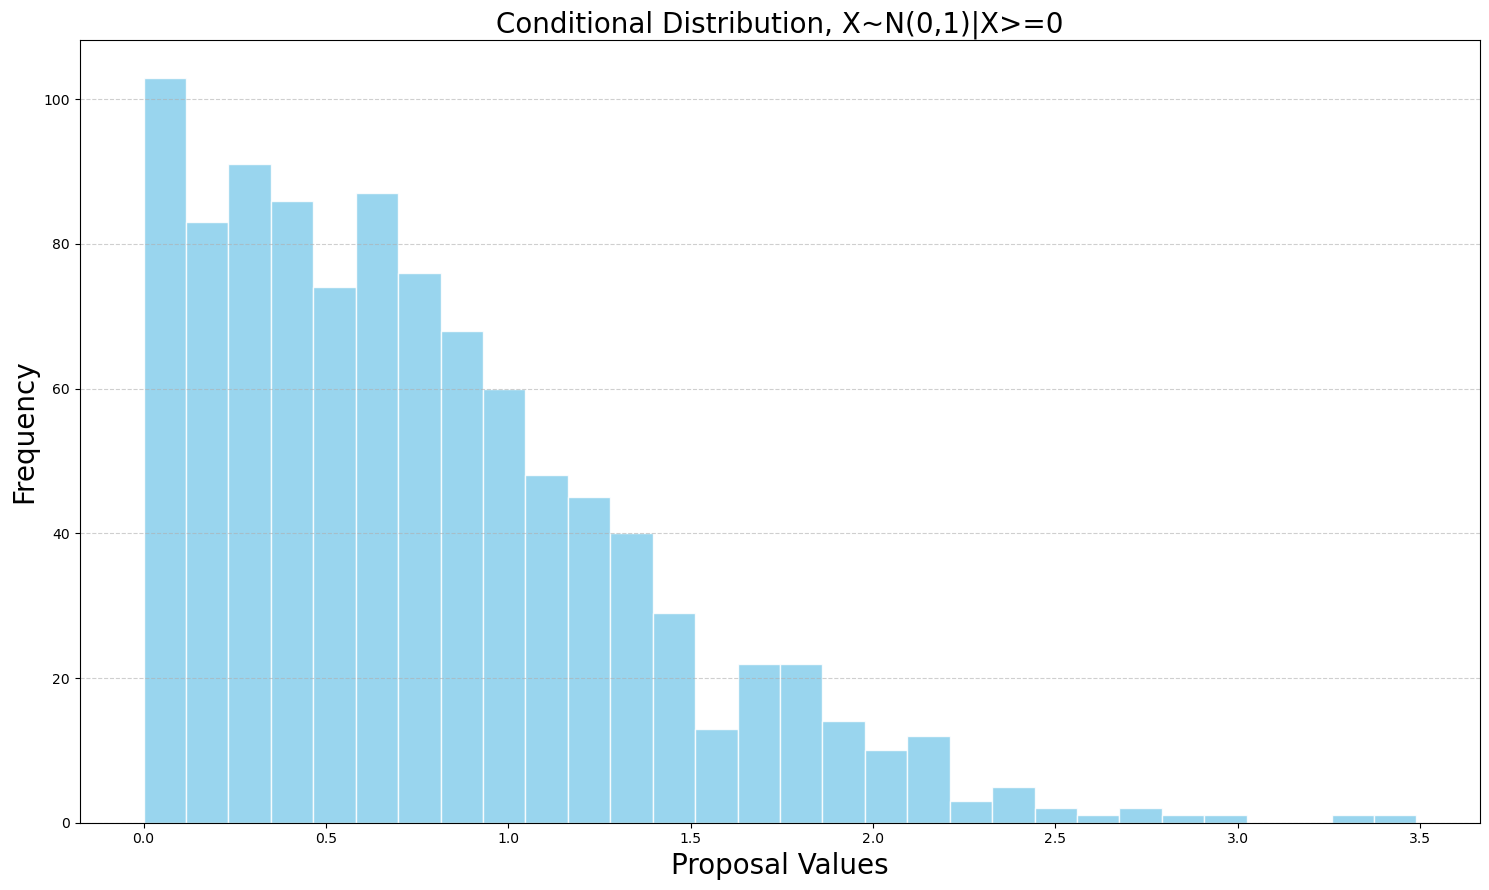
\includegraphics[scale=0.6]{chapter1-part4-plot1.png}
\end{center}
\end{frame}

%-------------------
% Slide 5: Conditional Distributions
%-------------------
\begin{frame}{Conditional Distributions}
\textbf{Remarks}

\vspace{3mm}

\begin{itemize}
	\item The described method to generate samples from conditional distributions is very straightforward as long as we know how to sample from the unconditional distribution of $X$.
	\item The proposals will be accepted with probability $P(A)$ so the efficiency of the method may not be good if $A$ is an event with very low probability.
	\item In cases where $P(A)$ is small, this method might not be advisable. Example 1.28 from the textbook covers one of such examples and provides an alternative solution.
\end{itemize}
\end{frame}


%-------------------
% Slide 6: Conditional Distributions
%-------------------
\begin{frame}{Rejection Sampling in Arbitrary Spaces}
\textbf{Rejection Sampling in Arbitrary Spaces}

\vspace{2mm}

One of the advantages of rejection sampling is that it can be used to generate random objects in more general spaces, in particular random vectors.

\vspace{2mm}

A standard use of the rejection sampling algorithm is related to the generation of uniformly distributed random vectors over some arbitrary subsets of $\mathbb{R}^d$.

\vspace{2mm}

For simplicity we will focus on the case $d=2$ (which can be visualized easily) but these ideas also apply in higher dimensions.
\end{frame}

%-------------------
% Slide 6: Uniform sampling from a rectangle
%-------------------
\begin{frame}{Rejection Sampling in Arbitrary Spaces}
\textbf{Uniform sampling from a rectangle}

\vspace{2mm}

If we want to generate a random vector with uniform distribution over the rectangle $[a,b]\times[c,d]$ we can do so directly by generating its two components independently one from the other (each of them uniformly distributed) as follows:
\vspace{2mm}

\alert{Algorithm}:

\begin{enumerate}
\item Generate $X \sim U[a,b]$
\item Generate $Y \sim U[c,d]$ (independently of X)
\item Return vector $(X.Y)$
\end{enumerate}
\end{frame}

%-------------------
% Slide 7: Uniform sampling from a rectangle
%-------------------
\begin{frame}{Uniform sampling from a rectangle}
Plot of 500 uniformly distributed random points on $[0,2]\times[1,4]$.

\begin{center}
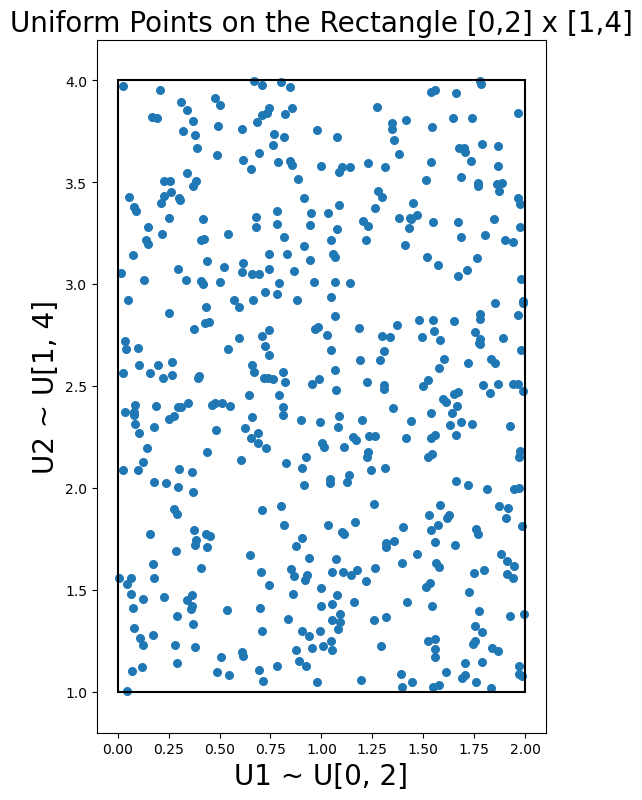
\includegraphics[scale=0.5]{chapter1-part4-plot2.png}
\end{center}
\end{frame}

%-------------------
% Slide 8: Conditional Distribution and Uniform Sampling
%-------------------
\begin{frame}{Rejection Sampling in Arbitrary Spaces}
\textbf{Main result}

\vspace{2mm}

\textbf{Lemma 1.31 from textbook}: Let $X$ be uniformly distributed on a set $A$, and let $B$ be a set such that $|A \cap B| >0$. Then the conditional distribution $P_{X| X \in B}$ of $X$ conditioned on the event $X \in B$ coincides with the uniform distribution on $A \cap B$.

\vspace{2mm}

\textbf{Remark}: The symbol $ |Y| $ refers to the ``volume'' (or measure) of set $Y$. For instance, In the case of two dimensions we need that the area of $A\cap B$ is strictly positive. 
\end{frame}

%-------------------
% Slide 9: Conditional Distribution and Uniform Sampling
%-------------------
\begin{frame}{Rejection Sampling in Arbitrary Spaces}
\begin{itemize}
	\item The previous Lemma indicates a possible approach (using rejection sampling) to generate random  vectors uniformly distributed in some ``irregular'' subset $B$ of $\mathbb{R}^2$ (and $\mathbb{R}^d$ in general).
	\item First we would need to start with a set $A \supset B$ so that we can sample uniformly distributed random vectors from $A$.
Then we will reject all the vectors that do not belong to $B$ and keep the generated random vectors in $B$. 
	\item According to the previous Lemma, this sample will be uniformly distributed on $A\cap B=B$.
	\item The easiest approach (but not strictly necessary or possible)
consists on selecting $A$ with a rectangular shape, as we already know how to generate random vectors from a rectangle.
\end{itemize} 
\end{frame}

%-------------------
% Slide 10: Conditional Distribution and Uniform Sampling
%-------------------
\begin{frame}{Rejection Sampling in Arbitrary Spaces Example}
\textbf{Example}: Generate a sample of uniformly distributed random vectors on the semicircle defined by $x^2+y^2\leq 1$ and $y\geq 0$.

\vspace{2mm}
\pause

\textbf{Solution}: We will use the algorithm described earlier with $B$ being the described semicircle and $A$ being the rectangle $[-1,1]\times [0,1]$ which includes $B$.

\vspace{2mm}

Essentially we will start generating uniformly distributed random numbers in the rectangle $A$ and out of those, we will reject the ones that are not in $B$. Notice that the theoretical probability that a proposal point is accepted is $\pi/4 \approx 0.785$. 
\end{frame}

%-------------------
% Slide 11: Algorithm: Rejection Sampling Inside Unit Semicircle
%-------------------
\begin{frame}[fragile]{Algorithm: Rejection Sampling Inside Unit Semicircle}
\begin{algorithm}[H]
    \caption{Generate points $(X_1, X_2)$ uniformly inside the semicircle}
    \begin{algorithmic}[1]
        \State \textbf{Input:} Integer $n$
        \State Initialize empty vectors $X_1$ and $X_2$
        \State Generate uniform random vectors:
        \Statex \quad $U_1 \sim \text{Uniform}(-1,1)^n$, $U_2 \sim \text{Uniform}(0,1)^n$
        \State Initialize counter: $\text{counter} \gets 1$
        \For{$i = 1$ to $n$}
            \If{$U_1[i]^2 + U_2[i]^2 < 1$}
                \State $X_1[\text{counter}] \gets U_1[i]$
                \State $X_2[\text{counter}] \gets U_2[i]$
                \State $\text{counter} \gets \text{counter} + 1$
            \EndIf
        \EndFor
        \State \textbf{Output:} $X_1, X_2$ (accepted points inside the semicircle)
    \end{algorithmic}
\end{algorithm}
\end{frame}

%-------------------
% Slide 12: Algorithm: Vectorized Rejection Sampling Inside Unit Semicircle
%-------------------
\begin{frame}[fragile]{Algorithm: Vectorized Rejection Sampling Inside Unit Semicircle}
\begin{algorithm}[H]
    \caption{Generate $n$ points $(X_1, X_2)$ uniformly inside the semicircle (vectorized)}
    \begin{algorithmic}[1]
        \State \textbf{Input:} Integer $n$
        \State Generate candidate points:
        \Statex \quad $U_1 \gets \text{runif}(n \times 2, -1, 1)$
        \Statex \quad $U_2 \gets \text{runif}(n \times 2, 0, 1)$
        \State Compute mask for points inside the unit circle:
        \Statex \quad $\text{inside} \gets (U_1^2 + U_2^2 < 1)$
        \State Keep only the accepted points:
        \Statex \quad $X_1 \gets U_1[\text{inside}]; X_1 \gets X_1[1:n]$
        \Statex \quad $X_2 \gets U_2[\text{inside}]; X_2 \gets X_2[1:n]$
        \State \textbf{Output:} $X_1, X_2$ (vectors of $n$ points inside the semicircle)
    \end{algorithmic}
\end{algorithm}

\textbf{Note}: In vectorized rejection sampling, we often generate more candidate points than needed (e.g., $n\times 2$) to ensure that enough points satisfy the acceptance condition. Since only a fraction of the candidates fall inside the desired region, oversampling increases the likelihood that we can select exactly $n$ accepted points without looping. The factor 2 is a simple heuristic; larger factors may be needed if the acceptance rate is low.
\end{frame}

%-------------------
% Slide 13: Results for Rejection Sampling Inside Unit Semicircle
%-------------------
\begin{frame}
The code gave us 780 generated uniformly distributed random points on the semicircle $x^2+y^2\leq 1$, $y\geq 0$. 

\begin{center}
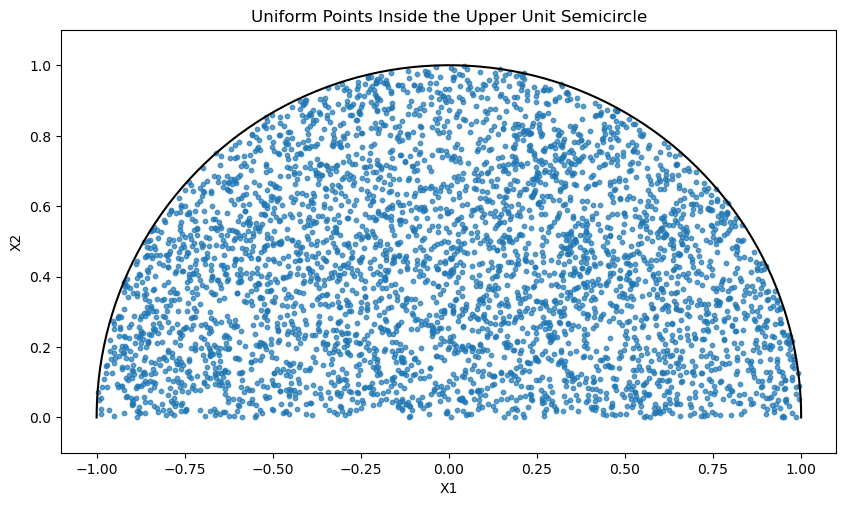
\includegraphics[scale=0.5]{chapter1-part4-plot3.png}
\end{center}
\end{frame}

%-------------------
% Slide 14: Remarks
%-------------------
\begin{frame}{Remarks}
\begin{itemize}
	\item As the previous example shows, this method can be very useful to generate samples that follow the uniform distribution over some irregular  sets of $\mathbb{R}^d$.
	\item If the set $B$ is small compared to the set $A$ then the method may be inefficient.
	\item It is better to use this method if we have a relatively easy way to check whether a given point belongs to set $B$ . That is easy for a semicircle(previous example) but not so easy if $B$ is a pentagram(a five-pointed star).
	\item Hard (but not impossible) to use this method if the set $B$ is unbounded, as we won't be able to enclose it in a rectangle $A$.
\end{itemize}
\end{frame}

%-------------------
% Slide 15: Homework
%-------------------
\begin{frame}{Homework}
\begin{enumerate}
	\item Write code for the uniform sampling from a rectangle algorithm, with $X \sim U[0,2]$ and $Y \sim U[1,4]$.
	\item Implement code for Algorithms 1 and 2 using the rectangle $[-1,1] \times [0,1]$. If computationally feasible, run both algorithms for $num\_sims = [50, 100, 500, 1000, 2000]$ and plot the difference in their running times.
		\begin{itemize}
	          \item \textbf{Hint:} Use built-in timers to measure running time:
	          \begin{itemize}
	              \item In Python: \texttt{import time; start = time.time(); ...; end = time.time()}
	              \item In R: \texttt{system.time(\{ ... \})}
	          \end{itemize}
	      \end{itemize}
	\item Write a computer program to generate a random sample of size 1000 from the conditional distribution of $X \sim Binomial(n,p)$  (with $n=10$ and probability of success $p=0.6$) conditioned on $X\geq 5$. 
	\item Write a computer program to generate (and plot) a sample of 500 uniformly distributed random points on the set of plane given by $y\geq 0$, $-\pi/2 \leq  x \leq \pi/2$, and $y \leq \cos x$.
\end{enumerate}
\end{frame}


\end{document}